\documentclass[11pt]{article}

\usepackage[a4paper,margin=1in]{geometry}
\usepackage{amsmath,amssymb,amsthm}
\usepackage{mathtools}
\usepackage{booktabs}
\usepackage{array}
\usepackage{xcolor}
\usepackage[hidelinks]{hyperref}
\usepackage{enumitem}
\usepackage{tikz}
\usetikzlibrary{matrix,positioning,fit,backgrounds,calc,decorations.pathreplacing}

\setlength{\parskip}{0.4em}
\setlength{\parindent}{0pt}

% ---- shared colours for the illustrations -------------------------------------------------------
\definecolor{laneA}{RGB}{31,119,180}   % lane a  (blue)
\definecolor{laneB}{RGB}{230,126,34}   % lane b  (orange)
\definecolor{iscol}{RGB}{120,120,120}  % initialization sequence (grey)
\definecolor{probe}{RGB}{39,174,96}    % the probe class (green)
\definecolor{softA}{RGB}{209,229,240}
\definecolor{softB}{RGB}{253,224,196}
\definecolor{softP}{RGB}{212,239,223}

\tikzset{
  cell/.style={draw,minimum width=1.05cm,minimum height=0.72cm,font=\small,inner sep=1pt},
  acell/.style={cell,fill=softA},
  bcell/.style={cell,fill=softB},
  iscell/.style={cell,fill=iscol!25,font=\small\bfseries},
  pcell/.style={cell,line width=1pt,draw=probe},
}

\theoremstyle{definition}
\newtheorem{definition}{Definition}
\newtheorem{assumption}{Assumption}
\newtheorem{remark}{Remark}
\newtheorem{example}{Example}

\theoremstyle{plain}
\newtheorem{lemma}{Lemma}
\newtheorem{theorem}{Theorem}
\newtheorem{corollary}{Corollary}
\newtheorem{proposition}{Proposition}

\newcommand{\ct}{\mathrm{ct}}
\newcommand{\run}{\mathrm{run}}
\newcommand{\boost}{\mathrm{boost}}
\newcommand{\IS}{\mathrm{IS}}
\newcommand{\HL}{H_{\mathrm{L1D}}}
\newcommand{\HF}{H_{\mathrm{full}}}
\newcommand{\Htr}{H}                     % a generic hardware trace (either HF or HL)
\newcommand{\lane}[1]{L^{(#1)}}
\newcommand{\inp}[2]{i_{#1}^{(#2)}}
\newcommand{\dprobe}{d}
\newcommand{\tmax}{t_{\max}}

\title{Generalized priming: why it is needed and why it is correct}
\author{Gal Kaptsenel}
\date{\today}

\begin{document}
\maketitle

\begin{abstract}
We show two things about Revizor's priming step. First, the current implementation
cannot report a whole class of genuine leaks: the ones whose only footprint falls
outside the cache the tool reads. This is a property of the priming decision rule, not
of any particular test case, and the canonicality leak we found is a concrete member
of the class. Second, the proposed generalization does not change the violation
definition, it only changes the methodology. It detects every leak the current tool
detects and strictly more, and its localization step provably returns a genuine
leaking input pair, distinguished by one and the same probe. We give two localizers, a
linear scan and a binary search, and prove each optimal for what it returns.
\end{abstract}

% #################################################################################################
\section{Definitions}
\label{sec:defs}

This section fixes every object the rest of the note uses; nothing here is proved. The
proofs start in Section~\ref{sec:limitation}.

\begin{definition}[Run and batch]
\label{def:batch}
A \emph{test case} $T$ is a fixed program. An \emph{input} $i$ sets the initial
architectural state of the sandbox. A \emph{run} starts from a microarchitectural
state $\mu$, executes $T$ on $i$, and ends in a new microarchitectural state; we write
$\run(T,i,\mu)$. A \emph{batch} runs a sequence of inputs in order. Before each run the
architectural sandbox is set explicitly, but the microarchitectural state is
\emph{carried over}: the state entering a run is the one the previous run left behind.
This carry-over is the only channel from one run to the next, and it flows only forward
in time.
\end{definition}

\begin{definition}[Initialization sequence]
\label{def:is}
An \emph{initialization sequence} $\IS$ is a fixed routine whose job is to drive the
microarchitectural state into one fixed, reproducible value $\mu_\IS$, regardless of
what ran earlier.
\end{definition}

\begin{definition}[Traces]
\label{def:traces}
The \emph{contract trace} $\ct(T,i)$ is the leakage the reference contract permits for
$i$ under $T$; it depends on $T$ and $i$ only. A run also leaves a microarchitectural
footprint, and a \emph{hardware trace} is the part of it an attacker reads. We name a
generic hardware trace $\Htr$, and two concrete ones matter here.
\begin{itemize}[nosep,leftmargin=1.4em]
\item $\HL$ --- the L1D cache trace measured by Prime+Probe or Flush+Reload, the
      hardware trace Revizor uses today.
\item $\HF$ --- the \emph{full} leftover a run leaves, of which $\HL$ is one
      projection: anything $\HL$ separates, $\HF$ separates too, but not conversely.
\end{itemize}
\end{definition}

\begin{definition}[Violation]
\label{def:violation}
A \emph{violation} is a tuple $(T,i_0,i_1,\mu)$ --- a test case $T$, two distinct
inputs $i_0,i_1$, and a common microarchitectural state $\mu$ --- such that the
contract cannot tell the inputs apart yet the hardware does:
\[
  \ct(T,i_0)=\ct(T,i_1)
  \qquad\text{and}\qquad
  \Htr(\run(T,i_0,\mu))\neq \Htr(\run(T,i_1,\mu)).
\]
The faithful trace here is $\Htr=\HF$; Revizor approximates it by its projection
$\Htr=\HL$.
\end{definition}

\begin{definition}[Priming, the current decision rule]
\label{def:prime}
Take a batch $i_0,i_1,\dots,i_k$ and write $\mu_p$ for the state reached after running
$i_0,\dots,i_{p-1}$ (so input $i_p$ runs from $\mu_p$). Revizor \emph{flags a suspected
violation} between two same-class inputs $i_a,i_b$ when they leave different L1D traces
in their own slots:
\[
  \ct(T,i_a)=\ct(T,i_b)
  \qquad\text{and}\qquad
  \HL(\run(T,i_a,\mu_a))\neq \HL(\run(T,i_b,\mu_b)).
\]
\emph{Priming} then equalizes history: it swaps the two inputs into each other's slot
and re-measures each candidate against the other from a \emph{common} preceding state.
This yields two equalized comparisons,
\[
  \underbrace{\HL(\run(T,i_a,\mu_a))\;\text{vs.}\;\HL(\run(T,i_b,\mu_a))}_{\text{both from }\mu_a}
  \qquad
  \underbrace{\HL(\run(T,i_a,\mu_b))\;\text{vs.}\;\HL(\run(T,i_b,\mu_b))}_{\text{both from }\mu_b}.
\]
Priming \emph{keeps} the finding if at least one comparison still differs, and
\emph{discards} it (declares a false positive) when both agree:
\[
  \HL(\run(T,i_a,\mu_a))=\HL(\run(T,i_b,\mu_a))
  \quad\text{and}\quad
  \HL(\run(T,i_a,\mu_b))=\HL(\run(T,i_b,\mu_b)).
\]
\end{definition}

\begin{definition}[Noncache violation]
\label{def:xio}
A violation $(T,i_0,i_1,\mu)$ (Definition~\ref{def:violation}) is \emph{noncache} when
\begin{enumerate}[label=(\alph*),nosep,leftmargin=2.2em]
\item for every microarchitectural state $\mu'$,
      $\HL(\run(T,i_0,\mu')) = \HL(\run(T,i_1,\mu'))$ --- the choice between $i_0$ and
      $i_1$ never changes the L1D trace of its \emph{own} run; and
\item for some $\mu''$, $\HF(\run(T,i_0,\mu'')) \neq \HF(\run(T,i_1,\mu''))$ --- the two
      do leave different \emph{full} footprints.
\end{enumerate}
\end{definition}

\begin{definition}[Input class]
\label{def:class}
Fix a test case $T$ and contract trace $\ct$. Two inputs $i_0,i_1$ are in the same
\emph{class} when they share a contract trace, $\ct(T,i_0)=\ct(T,i_1)$. A class is thus
a set of inputs the contract deems indistinguishable.
\end{definition}

\begin{definition}[Boosting]
\label{def:boost}
Revizor \emph{boosts} an input $i$ (under $T$) by generating other inputs of the same
class as $i$ (Definition~\ref{def:class}) --- distinct inputs with the identical
contract trace.
\end{definition}

\begin{definition}[Lane]
\label{def:lane}
A \emph{lane} is a batch that holds one input from each of $k+1$ classes:
$\lane{\ell}=(\inp{0}{\ell},\dots,\inp{k}{\ell})$, where $\inp{m}{\ell}$ is its member
of class $m$. Two lanes $a,b$ therefore meet class $m$ with two \emph{different} inputs
$\inp{m}{a},\inp{m}{b}$ that still share the contract trace of class $m$; boosting is
what supplies the second member. Revizor runs lanes one after another, each preceded by
$\IS$ (Definition~\ref{def:is}):
\end{definition}

\begin{center}
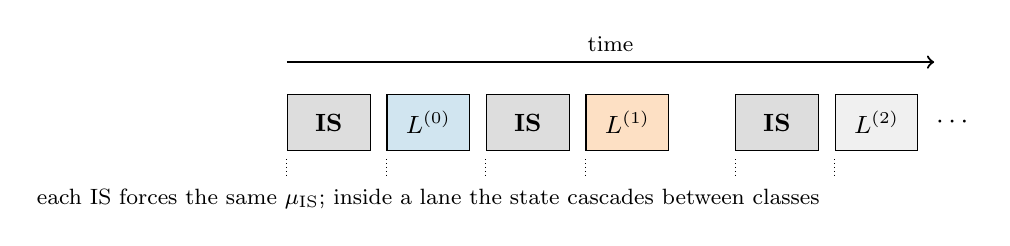
\begin{tikzpicture}[node distance=2mm]
  \node[iscell] (is0) {IS};
  \node[acell,right=of is0] (l0) {$\lane{0}$};
  \node[iscell,right=of l0] (is1) {IS};
  \node[bcell,right=of is1] (l1) {$\lane{1}$};
  \node[iscell,right=of is1,xshift=1.9cm] (is2) {IS};
  \node[cell,fill=black!6,right=of is2] (l2) {$\lane{2}$};
  \node[right=1mm of l2] (dots) {$\cdots$};
  \draw[->,thick] ($(is0.north west)+(0,4mm)$) -- ($(l2.north east)+(2mm,4mm)$)
        node[midway,above,font=\footnotesize] {time};
  \foreach \n in {is0,l0,is1,l1,is2,l2}{\draw[densely dotted] (\n.south west)+(0,-1mm) -- +(0,-3mm);}
  \node[font=\footnotesize,align=center] at ($(l0.south)+(0,-6mm)$)
        {each IS forces the same $\mu_\IS$; inside a lane the state cascades between classes};
\end{tikzpicture}
\end{center}

\paragraph{The matrix picture.}
Stack the lanes as the rows of a matrix and let the classes be its columns. Entry
$(\ell,m)$ is the input $\inp{m}{\ell}$. A lane is a row, read left to right; running it
means $\IS$, then the row's inputs in column order, with the microarchitectural state
cascading along the row.
\[
  M \;=\;
  \begin{array}{c|cccc}
     & \text{class }0 & \text{class }1 & \cdots & \text{class }k \\ \hline
    \text{lane }a & \inp{0}{a} & \inp{1}{a} & \cdots & \inp{k}{a} \\
    \text{lane }b & \inp{0}{b} & \inp{1}{b} & \cdots & \inp{k}{b} \\
    \vdots        &            &            &        &            \\
  \end{array}
\]
Every column is one class, so the contract cannot tell its entries apart. Any $\HL$
difference between two rows read at the \emph{same} column is therefore, by definition,
a violation candidate.

\paragraph{Convention: the detecting class is the last one.}
Suppose a candidate is flagged at class $\dprobe$ (two rows disagree at column
$\dprobe$). A run at a later column happens \emph{after} the class-$\dprobe$ run, and
carry-over flows only forward (Definition~\ref{def:batch}), so no later column can
change the class-$\dprobe$ reading. We may drop every column after $\dprobe$ and relabel
so the detecting class is the last one, $k$. From here on we call class $k$ the
\emph{probe}.

\begin{definition}[Prefix/suffix splice]
\label{def:toggle}
For two lanes $a,b$ and a split $t\in\{0,\dots,k+1\}$, the splice $\sigma_{a\to b}(t)$
is the row that takes columns \emph{before} $t$ from lane $a$ and columns \emph{from}
$t$ \emph{on} from lane $b$:
\[
  \sigma_{a\to b}(t)=\bigl(\underbrace{\inp{0}{a},\dots,\inp{t-1}{a}}_{\text{prefix: lane }a},\
                           \underbrace{\inp{t}{b},\dots,\inp{k}{b}}_{\text{suffix: lane }b}\bigr).
\]
So $\sigma_{a\to b}(0)=\lane{b}$ (all $b$) and $\sigma_{a\to b}(k+1)=\lane{a}$ (all
$a$). Two neighbours $\sigma_{a\to b}(t)$ and $\sigma_{a\to b}(t+1)$ are the same row
except at column $t$: they share the prefix (columns $<t$, from $a$) and the whole
suffix (columns $>t$, from $b$, probe included), and differ only in the input at column
$t$. Each splice is run as a batch $\IS,\sigma_{a\to b}(t)$, so both neighbours also
share the same start $\mu_\IS$.
\end{definition}

\begin{center}
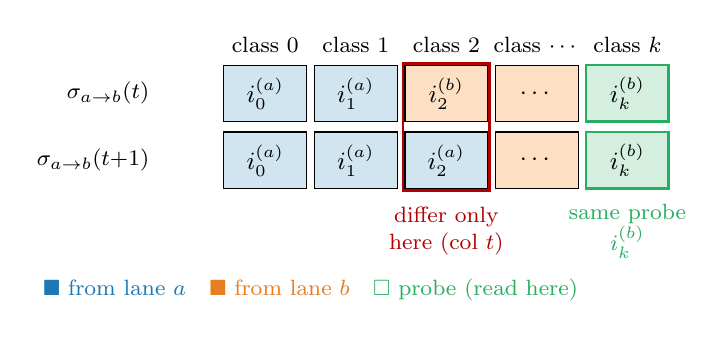
\begin{tikzpicture}[node distance=0mm,font=\small]
  \foreach \c/\lab in {0/0,1/1,2/2,3/{\cdots},4/k}{
     \node[font=\footnotesize] at (\c*1.15,0.62) {class $\lab$};}
  \node[left=2mm of {(-0.575,0)},font=\footnotesize] at (-1.15,0) {$\sigma_{a\to b}(t)$};
  \node[acell] at (0,0) {$\inp{0}{a}$};
  \node[acell] at (1.15,0) {$\inp{1}{a}$};
  \node[bcell] at (2.3,0) {$\inp{2}{b}$};
  \node[cell,fill=softB] at (3.45,0) {$\cdots$};
  \node[pcell,fill=softP] at (4.6,0) {$\inp{k}{b}$};
  \node[left=2mm of {(-0.575,-0.85)},font=\footnotesize] at (-1.15,-0.85) {$\sigma_{a\to b}(t{+}1)$};
  \node[acell] at (0,-0.85) {$\inp{0}{a}$};
  \node[acell] at (1.15,-0.85) {$\inp{1}{a}$};
  \node[acell] at (2.3,-0.85) {$\inp{2}{a}$};
  \node[cell,fill=softB] at (3.45,-0.85) {$\cdots$};
  \node[pcell,fill=softP] at (4.6,-0.85) {$\inp{k}{b}$};
  \draw[red!70!black,line width=1pt] (2.3-0.55,0.38) rectangle (2.3+0.55,-0.85-0.38);
  \node[red!70!black,font=\footnotesize,align=center] at (2.3,-1.75)
       {differ only\\ here (col $t$)};
  \node[probe,font=\footnotesize,align=center] at (4.6,-1.75) {same probe\\ $\inp{k}{b}$};
  \node[font=\footnotesize] at (0.575,-2.5) {\textcolor{laneA}{$\blacksquare$ from lane $a$}\quad
       \textcolor{laneB}{$\blacksquare$ from lane $b$}\quad
       \textcolor{probe}{$\square$ probe (read here)}};
\end{tikzpicture}
\end{center}

\begin{definition}[Splice measurement]
\label{def:measure}
To \emph{measure the splice} at split $t$: run the batch $\IS,\sigma_{a\to b}(t)$ and read
the L1D trace of its class-$k$ (probe) run. Let $\mu_t$ be the microarchitectural state
that $\IS$ and classes $0,\dots,k-1$ of $\sigma_{a\to b}(t)$ leave, and $c_t$ the class-$k$
input the splice carries ($c_t=\inp{k}{a}$ when $t=k+1$, otherwise $c_t=\inp{k}{b}$). The
splice measurement is
\[
  r(t)=\HL(\run(T,\,c_t,\,\mu_t)).
\]
\end{definition}

\clearpage

% #################################################################################################
\section{The limitation}
\label{sec:limitation}

\paragraph{Intuition.}
An input can \emph{write} a microarchitectural resource $X$ that its own run never
\emph{reads back} into the cache. Then that write leaves no mark on the run's own
$\HL$; it survives only as leftover and shows up, if at all, in a \emph{later} run that
does read $X$. Current priming was built to erase exactly this kind of carried-over
effect, so it erases the evidence of such a leak along with the noise.

\begin{center}
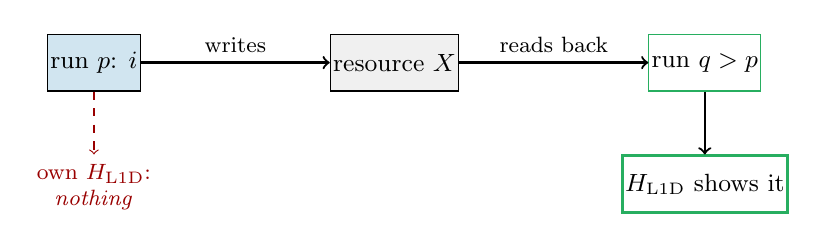
\begin{tikzpicture}[node distance=6mm,font=\small]
  \node[acell] (rp) {run $p$: $i$};
  \node[cell,fill=black!6,right=2.4cm of rp] (X) {resource $X$};
  \node[cell,draw=probe,right=2.4cm of X] (rq) {run $q>p$};
  \node[pcell,below=8mm of rq] (l1) {$\HL$ shows it};
  \draw[->,thick] (rp) -- node[above,font=\footnotesize]{writes} (X);
  \draw[->,thick] (X) -- node[above,font=\footnotesize]{reads back} (rq);
  \draw[->,thick] (rq) -- (l1);
  \node[below=8mm of rp,font=\footnotesize,align=center,text=red!60!black]
        (no) {own $\HL$:\\ \emph{nothing}};
  \draw[->,red!60!black,dashed] (rp) -- (no);
\end{tikzpicture}
\end{center}

\begin{theorem}[Current priming misses noncache violations]
\label{thm:miss}
If a violation $(T,i_a,i_b,\mu)$ is noncache (Definition~\ref{def:xio}), the rule of
Definition~\ref{def:prime} never reports it.
\end{theorem}

\begin{proof}
A pair is reported only if it is first flagged as a suspected violation and then
survives priming, so it suffices to show priming always discards it. Suppose the pair
is flagged at slots $a,b$, with preceding states $\mu_a,\mu_b$. Priming runs the two
equalized comparisons of Definition~\ref{def:prime}. By noncache condition
\ref{def:xio}(a), applied at $\mu'=\mu_a$ and at $\mu'=\mu_b$,
\[
  \HL(\run(T,i_a,\mu_a))=\HL(\run(T,i_b,\mu_a))
  \quad\text{and}\quad
  \HL(\run(T,i_a,\mu_b))=\HL(\run(T,i_b,\mu_b)),
\]
so both comparisons agree. That is exactly the discard condition, so priming declares a
false positive and the pair is never reported.
\end{proof}

\begin{remark}
Theorem~\ref{thm:miss} is unconditional: it uses nothing about the channel or the test
case, only the shape of the priming rule. Priming was introduced to discard differences
caused by carried-over state, and a noncache violation is visible, if at all, only
through carried-over state --- so the rule discards it by construction.
\end{remark}

The canonicality leak is such a violation. A BTB entry is indexed by (a subset of) a
branch's PC bits. Revizor's test cases are loop-free, so within one run a given branch
executes once: its BTB entry can be written but not re-read in the same run. Any
information the input pushes into that entry, and that the cache cannot see by other
means, therefore changes $\HF$ but not the run's own $\HL$. Conditions \ref{def:xio}(a)
and (b) hold, and by Theorem~\ref{thm:miss} current priming cannot report it. The branch
history, the prefetcher, the TLB, the pattern history table and the return stack all
supply the same kind of $X$.

% #################################################################################################
\section{Localizing the leak}
\label{sec:localize}

We keep Definition~\ref{def:violation} unchanged and only change the methodology. The
key move is to \emph{observe the leftover without reading it}: we never read $\HF$; we
let one input's leftover propagate into the cache of a later run and read it there.

Assume Revizor found input class $5$ from lanes $a$ and $b$ is a suspected violation, meaning, running lane $a$ and measuring input class $5$ returned a different $\HL$ from running lane $b$ and measuring at input class $5$. That is $r(k+1)=\HL(\run(T,\inp{5}{a}, \mu_5^{(a)}))\neq \HL(\run(T,\inp{5}{b}, \mu_5^{(b)}))=r(0)$ where $\mu_5^{(a)}$ is the microarch state resulted by running lane $a$ inputs prior to input class 5 and $\mu_5^{(b)}$  is the microarch state resulted by running lane $b$ inputs prior to input class 5.


\begin{center}
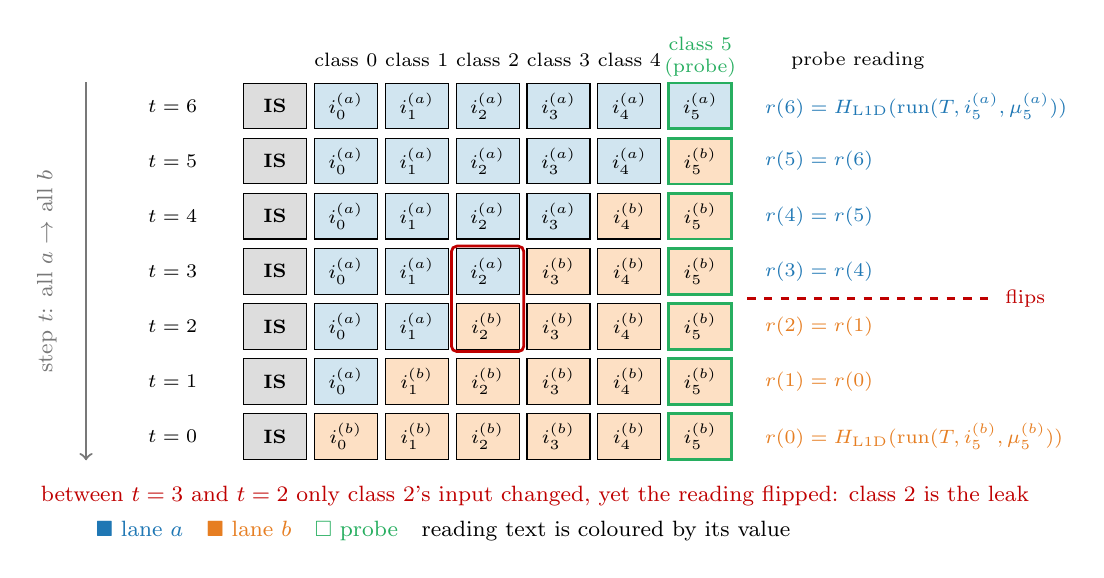
\begin{tikzpicture}[node distance=0mm,font=\small,
  ce/.style={draw,minimum width=0.8cm,minimum height=0.58cm,font=\scriptsize,inner sep=1pt},
  ca/.style={ce,fill=softA}, cb/.style={ce,fill=softB},
  ci/.style={ce,fill=iscol!25,font=\scriptsize\bfseries},
  cpa/.style={ce,line width=1pt,draw=probe,fill=softA},
  cpb/.style={ce,line width=1pt,draw=probe,fill=softB}]
  % headers
  \foreach \c/\x in {0/0.9,1/1.8,2/2.7,3/3.6,4/4.5}{\node[font=\scriptsize] at (\x,0.58) {class \c};}
  \node[probe,font=\scriptsize,align=center] at (5.4,0.62) {class 5\\(probe)};
  \node[font=\scriptsize] at (7.4,0.58) {probe reading};
  % t=6 : all a
  \node[font=\scriptsize] at (-1.3,0) {$t=6$};   \node[ci] at (0,0) {IS};
  \node[ca] at (0.9,0) {$\inp{0}{a}$}; \node[ca] at (1.8,0) {$\inp{1}{a}$};
  \node[ca] at (2.7,0) {$\inp{2}{a}$}; \node[ca] at (3.6,0) {$\inp{3}{a}$};
  \node[ca] at (4.5,0) {$\inp{4}{a}$}; \node[cpa] at (5.4,0) {$\inp{5}{a}$};
  \node[laneA,font=\scriptsize,anchor=west] at (6.1,0) {$r(6)=\HL(\run(T,\inp{5}{a},\mu_5^{(a)}))$};
  % t=5
  \node[font=\scriptsize] at (-1.3,-0.7) {$t=5$};   \node[ci] at (0,-0.7) {IS};
  \node[ca] at (0.9,-0.7) {$\inp{0}{a}$}; \node[ca] at (1.8,-0.7) {$\inp{1}{a}$};
  \node[ca] at (2.7,-0.7) {$\inp{2}{a}$}; \node[ca] at (3.6,-0.7) {$\inp{3}{a}$};
  \node[ca] at (4.5,-0.7) {$\inp{4}{a}$}; \node[cpb] at (5.4,-0.7) {$\inp{5}{b}$};
  \node[laneA,font=\scriptsize,anchor=west] at (6.1,-0.7) {$r(5)=r(6)$};
  % t=4
  \node[font=\scriptsize] at (-1.3,-1.4) {$t=4$};   \node[ci] at (0,-1.4) {IS};
  \node[ca] at (0.9,-1.4) {$\inp{0}{a}$}; \node[ca] at (1.8,-1.4) {$\inp{1}{a}$};
  \node[ca] at (2.7,-1.4) {$\inp{2}{a}$}; \node[ca] at (3.6,-1.4) {$\inp{3}{a}$};
  \node[cb] at (4.5,-1.4) {$\inp{4}{b}$}; \node[cpb] at (5.4,-1.4) {$\inp{5}{b}$};
  \node[laneA,font=\scriptsize,anchor=west] at (6.1,-1.4) {$r(4)=r(5)$};
  % t=3
  \node[font=\scriptsize] at (-1.3,-2.1) {$t=3$};   \node[ci] at (0,-2.1) {IS};
  \node[ca] at (0.9,-2.1) {$\inp{0}{a}$}; \node[ca] at (1.8,-2.1) {$\inp{1}{a}$};
  \node[ca] at (2.7,-2.1) {$\inp{2}{a}$}; \node[cb] at (3.6,-2.1) {$\inp{3}{b}$};
  \node[cb] at (4.5,-2.1) {$\inp{4}{b}$}; \node[cpb] at (5.4,-2.1) {$\inp{5}{b}$};
  \node[laneA,font=\scriptsize,anchor=west] at (6.1,-2.1) {$r(3)=r(4)$};
  % t=2 : reading flips here (vs t=3)
  \node[font=\scriptsize] at (-1.3,-2.8) {$t=2$};   \node[ci] at (0,-2.8) {IS};
  \node[ca] at (0.9,-2.8) {$\inp{0}{a}$}; \node[ca] at (1.8,-2.8) {$\inp{1}{a}$};
  \node[cb] at (2.7,-2.8) {$\inp{2}{b}$}; \node[cb] at (3.6,-2.8) {$\inp{3}{b}$};
  \node[cb] at (4.5,-2.8) {$\inp{4}{b}$}; \node[cpb] at (5.4,-2.8) {$\inp{5}{b}$};
  \node[laneB,font=\scriptsize,anchor=west] at (6.1,-2.8) {$r(2)=r(1)$};
  % t=1
  \node[font=\scriptsize] at (-1.3,-3.5) {$t=1$};   \node[ci] at (0,-3.5) {IS};
  \node[ca] at (0.9,-3.5) {$\inp{0}{a}$}; \node[cb] at (1.8,-3.5) {$\inp{1}{b}$};
  \node[cb] at (2.7,-3.5) {$\inp{2}{b}$}; \node[cb] at (3.6,-3.5) {$\inp{3}{b}$};
  \node[cb] at (4.5,-3.5) {$\inp{4}{b}$}; \node[cpb] at (5.4,-3.5) {$\inp{5}{b}$};
  \node[laneB,font=\scriptsize,anchor=west] at (6.1,-3.5) {$r(1)=r(0)$};
  % t=0 : all b
  \node[font=\scriptsize] at (-1.3,-4.2) {$t=0$};   \node[ci] at (0,-4.2) {IS};
  \node[cb] at (0.9,-4.2) {$\inp{0}{b}$}; \node[cb] at (1.8,-4.2) {$\inp{1}{b}$};
  \node[cb] at (2.7,-4.2) {$\inp{2}{b}$}; \node[cb] at (3.6,-4.2) {$\inp{3}{b}$};
  \node[cb] at (4.5,-4.2) {$\inp{4}{b}$}; \node[cpb] at (5.4,-4.2) {$\inp{5}{b}$};
  \node[laneB,font=\scriptsize,anchor=west] at (6.1,-4.2) {$r(0)=\HL(\run(T,\inp{5}{b},\mu_5^{(b)}))$};
  % step arrow
  \draw[->,thick,iscol] (-2.4,0.3) -- (-2.4,-4.5);
  \node[iscol,rotate=90,anchor=south,font=\footnotesize] at (-2.65,-2.1) {step $t$: all $a$ $\to$ all $b$};
  % culprit box: class 2 across t=3 and t=2
  \draw[red!75!black,line width=1pt,rounded corners=2pt]
        (2.7-0.46,-2.1+0.32) rectangle (2.7+0.46,-2.8-0.32);
  % flip marker across the readings
  \draw[red!75!black,line width=1pt,dashed] (6.0,-2.45) -- (9.1,-2.45);
  \node[red!75!black,font=\scriptsize,anchor=west] at (9.15,-2.45) {flips};
  % caption
  \node[red!75!black,font=\footnotesize,align=center] at (3.3,-4.95)
        {between $t=3$ and $t=2$ only class 2's input changed, yet the reading flipped: class 2 is the leak};
  % legend
  \node[font=\footnotesize,anchor=west] at (-2.4,-5.4)
     {\textcolor{laneA}{$\blacksquare$ lane $a$}\quad
      \textcolor{laneB}{$\blacksquare$ lane $b$}\quad
      \textcolor{probe}{$\square$ probe}\quad
      reading text is coloured by its value};
\end{tikzpicture}
\end{center}

Notice that the ends of the above ladder are exactly the measurements Revizor flagged (Definition~\ref{def:measure}), so they disagree;
hence the measurement must change at some step $t^\star$. A step where it changes is a \emph{boundary}.
In the above example, the boundary is $t^\star=2$.

Recall $r(t)$ is the splice measurement (Definition~\ref{def:measure}). Two facts about
boundaries settle everything: at least one exists (Proposition~\ref{prop:boundary}), and
each one is a genuine violation (Lemma~\ref{lem:genuine}).

\begin{proposition}[A boundary exists]
\label{prop:boundary}
Whenever the ends disagree ($r(k+1)\neq r(0)$), some split $t$ is a boundary.
\end{proposition}

\begin{proof}
Stepping gives the chain $r(0),r(1),\dots,r(k+1)$ with $r(0)\neq r(k+1)$ (the two ends
are the flagged candidate). If $r(t)=r(t+1)$ for all $t$ then $r(0)=\dots=r(k+1)$,
contradicting the ends. Hence $r(t)\neq r(t+1)$ for some $t$ --- a boundary.
\end{proof}

\begin{lemma}[Every boundary is a genuine violation; noncache when $\HL$-blind]
\label{lem:genuine}
Let $t$ be any boundary, i.e.\ $r(t)\neq r(t+1)$. Then $(T,\inp{t}{a},\inp{t}{b})$ is a
genuine violation (Definition~\ref{def:violation}). If moreover the pair is
indistinguishable in $\HL$ for all $\mu$, the violation is noncache.
\end{lemma}

The boundary is a single step, so the two batches around it differ in exactly one input;
after that input, the \emph{exact same routine} runs in both --- the identical suffix,
whose last run is the probe that is measured. That is what makes the returned pair a
genuine violation. We zoom into the two boundary rows $t=3$ and $t=2$ of the ladder
above:

\begin{center}
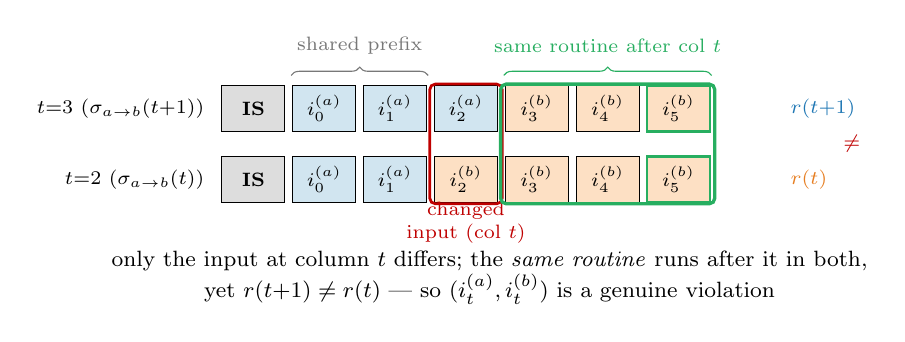
\begin{tikzpicture}[node distance=0mm,font=\small,
  ce/.style={draw,minimum width=0.8cm,minimum height=0.58cm,font=\scriptsize,inner sep=1pt},
  ca/.style={ce,fill=softA}, cb/.style={ce,fill=softB},
  ci/.style={ce,fill=iscol!25,font=\scriptsize\bfseries},
  cpb/.style={ce,line width=1pt,draw=probe,fill=softB}]
  % shared prefix brace (cols 0,1) above
  \draw[decorate,decoration={brace,amplitude=3pt},iscol] (0.9-0.42,0.42) -- (1.8+0.42,0.42);
  \node[iscol,font=\scriptsize] at (1.35,0.8) {shared prefix};
  % same-routine brace (cols 3..5, probe included) above
  \draw[decorate,decoration={brace,amplitude=3pt},probe] (3.6-0.42,0.42) -- (5.4+0.42,0.42);
  \node[probe,font=\scriptsize] at (4.5,0.8) {same routine after col $t$};
  % row sigma(t+1) = t=3
  \node[font=\scriptsize,anchor=east] at (-0.5,0) {$t{=}3$ ($\sigma_{a\to b}(t{+}1)$)};
  \node[ci] at (0,0) {IS};
  \node[ca] at (0.9,0) {$\inp{0}{a}$}; \node[ca] at (1.8,0) {$\inp{1}{a}$};
  \node[ca] at (2.7,0) {$\inp{2}{a}$}; \node[cb] at (3.6,0) {$\inp{3}{b}$};
  \node[cb] at (4.5,0) {$\inp{4}{b}$}; \node[cpb] at (5.4,0) {$\inp{5}{b}$};
  \node[laneA,font=\scriptsize,anchor=west] at (6.7,0) {$r(t{+}1)$};
  % row sigma(t) = t=2
  \node[font=\scriptsize,anchor=east] at (-0.5,-0.9) {$t{=}2$ ($\sigma_{a\to b}(t)$)};
  \node[ci] at (0,-0.9) {IS};
  \node[ca] at (0.9,-0.9) {$\inp{0}{a}$}; \node[ca] at (1.8,-0.9) {$\inp{1}{a}$};
  \node[cb] at (2.7,-0.9) {$\inp{2}{b}$}; \node[cb] at (3.6,-0.9) {$\inp{3}{b}$};
  \node[cb] at (4.5,-0.9) {$\inp{4}{b}$}; \node[cpb] at (5.4,-0.9) {$\inp{5}{b}$};
  \node[laneB,font=\scriptsize,anchor=west] at (6.7,-0.9) {$r(t)$};
  % differ-only box on column t (=class 2 here)
  \draw[red!75!black,line width=1pt,rounded corners=2pt]
        (2.7-0.46,0.31) rectangle (2.7+0.46,-0.9-0.31);
  \node[red!75!black,font=\scriptsize,align=center] at (2.7,-1.45) {changed\\ input (col $t$)};
  % same-routine box: suffix cols 3..5 (probe included)
  \draw[probe,line width=1.2pt,rounded corners=2pt]
        (3.6-0.46,0.31) rectangle (5.4+0.46,-0.9-0.31);
  % readings differ
  \node[red!75!black,font=\scriptsize] at (7.6,-0.45) {$\neq$};
  % caption
  \node[font=\footnotesize,align=center] at (3.0,-2.15)
     {only the input at column $t$ differs; the \emph{same routine} runs after it in both,\\
      yet $r(t{+}1)\neq r(t)$ --- so $(\inp{t}{a},\inp{t}{b})$ is a genuine violation};
\end{tikzpicture}
\end{center}

\begin{proof}
The neighbours $\IS,\sigma_{a\to b}(t)$ and $\IS,\sigma_{a\to b}(t+1)$ share the same
$\IS$ (start $\mu_\IS$), the prefix (columns $<t$, lane $a$) and the whole suffix
(columns $>t$, lane $b$, probe included) --- the same routine runs after column $t$ in
both; they differ only at column $t$. Their probe readings differ (that is the
boundary). So one and the same routine, run after an identical history except for the
single input at column $t$, already separates $\inp{t}{a}$ from $\inp{t}{b}$.

Hence $\inp{t}{a},\inp{t}{b}$ are distinct inputs of one class (they share a contract
trace); they run from a common preceding state (the shared $\IS$ and prefix), the
equalization Definition~\ref{def:prime} asks for; and they leave different
microarchitectural state behind, since it feeds the differing probe ($\HF$ differs).
That is a violation.

If in addition $\inp{t}{a},\inp{t}{b}$ have the same $\HL$ for all $\mu$, then
\ref{def:xio}(a) holds, and \ref{def:xio}(b) holds because localization has just
separated their downstream effect. The violation is noncache: unseen by current priming,
yet certified here through its effect on the probe, without ever reading $\HF$.
\end{proof}

Together the two facts settle correctness: a boundary always exists, and \emph{any}
boundary the sweep exposes is a genuine violation. So localization reduces to finding a
boundary --- the two localizers below differ only in \emph{which} boundary they return.

\begin{remark}[Several boundaries may exist]
\label{rem:multiple}
The chain $r(0),\dots,r(k+1)$ can change value more than once, so there may be several
boundaries --- up to $k+1$ of them --- each a distinct leaking class and each genuine by
Lemma~\ref{lem:genuine}. The linear scan can report them all; the binary search returns
just one.
\end{remark}

\begin{remark}[Self- vs.\ cross-input, from the boundary $t$]
\label{rem:selfcross}
The boundary column $t$ says \emph{what kind} of leak it is.
\begin{itemize}[nosep,leftmargin=1.4em]
\item $t=k$ (the probe column itself): the pair leaks about \emph{itself} --- swapping
      the probe input changes the probe reading in the ordinary, same-run way. This is a
      \emph{self-dependent} leak, the kind current priming already catches.
\item $t<k$: an \emph{earlier} class's input changes a \emph{later} reading --- a
      \emph{cross-input} leak, the noncache case that motivates this work.
\end{itemize}
A caller that wants only cross-input findings drops $t=k$ and keeps $t<k$; every kept
boundary is still genuine by Lemma~\ref{lem:genuine}.
\end{remark}

\paragraph{Both directions.}
Within one direction the probe is fixed, but which class actually reads the leftover
back into the cache can be lane-specific: perhaps only $\inp{k}{a}$ performs the
readout, or only some class in a lane-$a$ suffix. So we step both ways:
$a\to b$ probes with $\inp{k}{b}$ and a lane-$b$ suffix, $b\to a$ with $\inp{k}{a}$ and a
lane-$a$ suffix; running both covers either. Each direction is independently sound
(Lemma~\ref{lem:genuine}), so reporting a boundary found in either adds no false
positive.

\subsection{Linear scan}

\begin{definition}[Localization by linear scan]
\label{def:alg}
In direction $a\to b$:
\begin{enumerate}[label=\arabic*.,nosep,leftmargin=*]
\item Read $r(k+1)$ (all $a$). Then step down, $t=k,k-1,\dots,0$, reading
      $r(t)$.
\item After each step compare the neighbours $r(t)$ and $r(t+1)$: they come from the
      same batch $\IS,\sigma$ apart from the single input at column $t$.
\item Report the first (largest) $t$ with $r(t)\neq r(t+1)$ --- or every such $t$ if all
      leaking classes are wanted --- with the pair $\inp{t}{a},\inp{t}{b}$.
\end{enumerate}
Run the same in direction $b\to a$. Every reported pair is a genuine violation by
Lemma~\ref{lem:genuine}.
\end{definition}

\begin{remark}[Measurement]
\label{rem:measure}
A single probe reading is noisy, so each $r(t)$ is a \emph{repeated} measurement, and
two readings count as different only when they stay apart across the repetitions.
Enough repetitions push the noise down until $r(t)$ behaves as a stable value, which is
what the steps above compare. The other fact we use is architectural: the sandbox is
set before each run and each lane starts from $\mu_\IS$, so the only channel between
columns of a spliced batch is the forward microarchitectural cascade.
\end{remark}

\subsection*{Cost and a matching lower bound}

We measure a localizer by its \emph{runs}: one run executes one spliced batch and
returns its probe reading $r(t)$; the only promise is $r(0)\neq r(k+1)$. We drop the
constant repetition count (Remark~\ref{rem:measure}) and the factor two for the two
directions. Write $\tmax=\max\{t: r(t)\neq r(t+1)\}$, the largest leaking class.

\begin{proposition}[Cost of the scan]
\label{prop:scancost}
The top-down scan reads $r(k+1),r(k),\dots$ until the first change and returns $\tmax$;
in the worst case it uses $k+2$ runs.
\end{proposition}

\begin{proof}
Reading downward, the first $t$ with $r(t)\neq r(t+1)$ is the largest such $t$, and
along the way it has confirmed $r(t+1)=\dots=r(k+1)$, so no boundary lies above it. The
values read are $r(k+1),\dots,r(t)$, at most all $k+2$ of them (attained when
$\tmax=0$).
\end{proof}

\begin{theorem}[Finding $\tmax$ needs a linear scan]
\label{thm:lb-scan}
Any algorithm that always returns $\tmax$ makes at least $k$ runs in the worst case. The
scan is therefore optimal up to a constant.
\end{theorem}

\begin{proof}
Fix $t^\star\in\{0,\dots,k\}$ and the single-boundary chain $S_{t^\star}$ with
$r(x)=r_b$ for $x\le t^\star$ and $r(x)=r_a$ for $x>t^\star$ (two distinct values). Its
only boundary is $t^\star$, so $\tmax=t^\star$, and correctness forces the output
$t^\star$ on $S_{t^\star}$.

Suppose the algorithm leaves some $u\in(t^\star,k]$ unread. Build $S'$ from
$S_{t^\star}$ by setting $r(u)=c$ for a third value $c\notin\{r_a,r_b\}$. Since $S'$
agrees with $S_{t^\star}$ on every position read, the execution is identical and it
again outputs $t^\star$. But $u\le k$ gives $r(u+1)=r_a$, so $r(u)=c\neq r(u+1)$ is a
boundary above $t^\star$, whence $\tmax(S')\ge u>t^\star$: wrong. Hence every
$u\in(t^\star,k]$ is read, that is $k-t^\star$ runs; taking $t^\star=0$ gives at least
$k$.
\end{proof}

% #################################################################################################
\section{A logarithmic localizer: binary search}
\label{sec:bsearch}

The scan returns the largest leaking class. If any one leaking class suffices, a binary
search finds one far faster, using the same splices and the same probe. It keeps a
window $[\ell,h]$ whose ends disagree ($r(\ell)\neq r(h)$) and always narrows to a half
that still disagrees, so a boundary is trapped inside.

\begin{definition}[Localization by binary search]
\label{def:bsearch}
In direction $a\to b$, keep an interval $[\ell,h]$ with $r(\ell)\neq r(h)$; start
$\ell=0,h=k+1$, which holds by the candidate. While $h>\ell+1$, let
$m=\lfloor(\ell+h)/2\rfloor$, run $\IS,\sigma_{a\to b}(m)$, read $r(m)$, and
\begin{itemize}[nosep,leftmargin=*]
\item if $r(m)\neq r(\ell)$, set $h:=m$;
\item otherwise $r(m)=r(\ell)\neq r(h)$, so set $\ell:=m$.
\end{itemize}
When $h=\ell+1$, return $t=\ell$ with the pair $\inp{\ell}{a},\inp{\ell}{b}$.
\end{definition}

\begin{center}
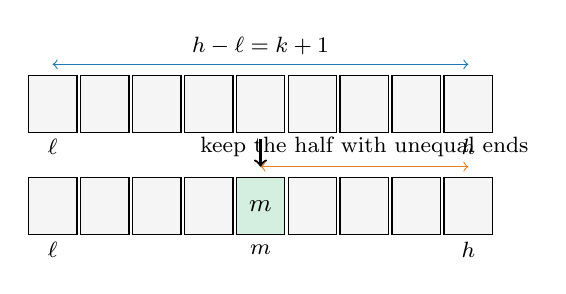
\begin{tikzpicture}[font=\footnotesize]
  \foreach \i in {0,...,8}{ \node[cell,minimum width=0.62cm,fill=black!4] (c\i) at (\i*0.66,0) {}; }
  \node at (0*0.66,-0.55) {$\ell$}; \node at (8*0.66,-0.55) {$h$};
  \draw[<->,laneA] (0*0.66,0.5) -- (8*0.66,0.5) node[midway,above,black]{$h-\ell=k+1$};
  \begin{scope}[yshift=-1.3cm]
  \foreach \i in {0,...,8}{ \node[cell,minimum width=0.62cm,fill=black!4] (d\i) at (\i*0.66,0) {}; }
  \node[cell,minimum width=0.62cm,fill=softP] at (4*0.66,0) {$m$};
  \draw[<->,laneB] (4*0.66,0.5) -- (8*0.66,0.5) node[midway,above,black]{keep the half with unequal ends};
  \node at (0*0.66,-0.55) {$\ell$}; \node at (4*0.66,-0.55) {$m$}; \node at (8*0.66,-0.55) {$h$};
  \end{scope}
  \draw[->,thick] (4*0.66,-0.45) -- (4*0.66,-0.8);
\end{tikzpicture}
\end{center}

\begin{proposition}[Binary search returns a genuine violation]
\label{prop:bsearch}
Binary search terminates after at most $\lceil\log_2(k+1)\rceil$ runs and returns a
boundary $t$. By Lemma~\ref{lem:genuine} the pair $\inp{t}{a},\inp{t}{b}$ is a genuine
violation.
\end{proposition}

\begin{proof}
The invariant $r(\ell)\neq r(h)$ holds initially and is preserved: if $r(m)\neq r(\ell)$
the new interval $[\ell,m]$ has unequal ends; otherwise $r(m)=r(\ell)$, and since
$r(\ell)\neq r(h)$ we get $r(m)\neq r(h)$, so $[m,h]$ has unequal ends. Each step halves
$h-\ell$, from $k+1$ to $1$, so it stops after at most $\lceil\log_2(k+1)\rceil$ reads
with $h=\ell+1$ and $r(\ell)\neq r(\ell+1)$, a boundary. Lemma~\ref{lem:genuine}
applies.
\end{proof}

Binary search returns \emph{some} leaking class, not necessarily $\tmax$, and it does
not enumerate the others; when that is all one needs, it is much cheaper.

\begin{theorem}[Finding any boundary needs a logarithmic search]
\label{thm:lb-bsearch}
Any algorithm that always returns some boundary makes at least $\lceil\log_2(k+1)\rceil$
runs in the worst case. Binary search is therefore optimal.
\end{theorem}

\begin{proof}
Use the single-boundary chains $S_j$, $j\in\{0,\dots,k\}$, with $r(x)=r_b$ for $x\le j$
and $r(x)=r_a$ for $x>j$; each satisfies $r(0)\neq r(k+1)$ and has its unique boundary
at $j$. Let $C$ be the set of $j$ still consistent with the answers so far; initially
$|C|=k+1$. A run at position $t$ returns $r_b$ for chains with $j\ge t$ and $r_a$ for
those with $j<t$, splitting $C$ into $\{j\in C: j\ge t\}$ and $\{j\in C: j<t\}$; the
adversary answers with the value of the larger part, so each run leaves $|C|$ at least
half its previous size. The algorithm may stop only when $|C|=1$: if two chains
$S_{j_1},S_{j_2}$ remain, its single output is the boundary of at most one, so it is
wrong on the other. Reducing $|C|$ from $k+1$ to $1$ by halving needs at least
$\lceil\log_2(k+1)\rceil$ runs.
\end{proof}

% #################################################################################################
\section{Comparison}

Both localizers use the same splices, the same probe comparison, and the same soundness
(Lemma~\ref{lem:genuine}); they differ in what they return and in cost. Entries are per
direction; multiply by two for both directions and by the repetition count of
Remark~\ref{rem:measure}.

\begin{center}
\begin{tabular}{@{}l p{4.6cm} p{4.6cm}@{}}
\toprule
 & \textbf{Linear scan} & \textbf{Binary search} \\
\midrule
Runs (worst case) & $k+2$ & $\lceil\log_2(k+1)\rceil$ \\[2pt]
Matching lower bound & $\ge k$ runs (Thm.~\ref{thm:lb-scan}) & $\ge \lceil\log_2(k+1)\rceil$ runs (Thm.~\ref{thm:lb-bsearch}) \\[2pt]
Returns & the largest leaking class $\tmax$; all leaking classes if continued & one leaking class (some boundary) \\[2pt]
Soundness & every returned pair is a genuine violation & every returned pair is a genuine violation \\[2pt]
Completeness & finds every leaking class & finds one, may miss others \\
\bottomrule
\end{tabular}
\end{center}

In short, current priming cannot report a noncache violation (Theorem~\ref{thm:miss}),
while the lane-toggle localization certifies one as a genuine violation, adhering to the
existing definitions, distinguished by one identical probe (Lemma~\ref{lem:genuine}).
The generalization keeps Definition~\ref{def:violation} and detects a strict superset.
When every leaking class is wanted, the linear scan is optimal (Theorem~\ref{thm:lb-scan});
when one suffices, binary search is optimal (Theorem~\ref{thm:lb-bsearch}).

\end{document}
